\chapter{Results}
\label{ch:results}
We show the results of the different experiments and discuss their implications.

\section{Experiment 1}
\subsection{Hyperparameter search}
After the first hyperparameter search, we found that the best $\alpha$ and $\lambda$ values appear in the bottom of the search range with good $\alpha$s ranging from 0.000001 to 0.0001 and $\lambda$s ranging from 0 to 0.15 (Fig.~\ref{fig:Hs1}).
\begin{figure}[h]
	\centering
	\begin{subfigure}{0.32\textwidth}
		\centering
                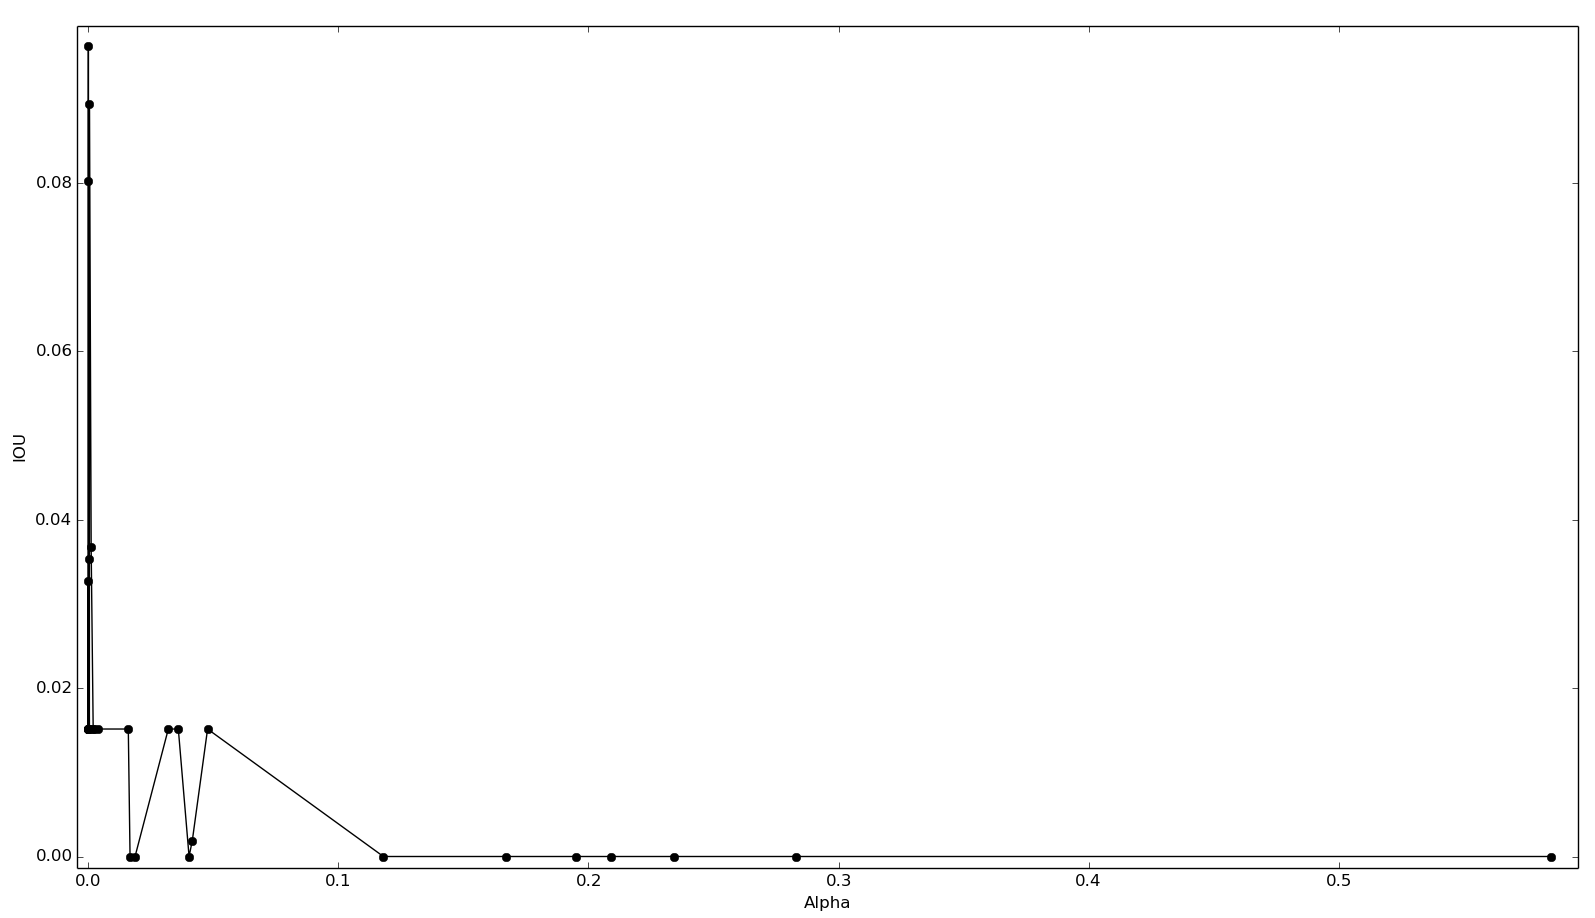
\includegraphics[width=\textwidth]{plots/hs1_alpha.png}
         \caption{IOU vs $\alpha$}
	\end{subfigure}
	\begin{subfigure}{0.32\textwidth}
		\centering
                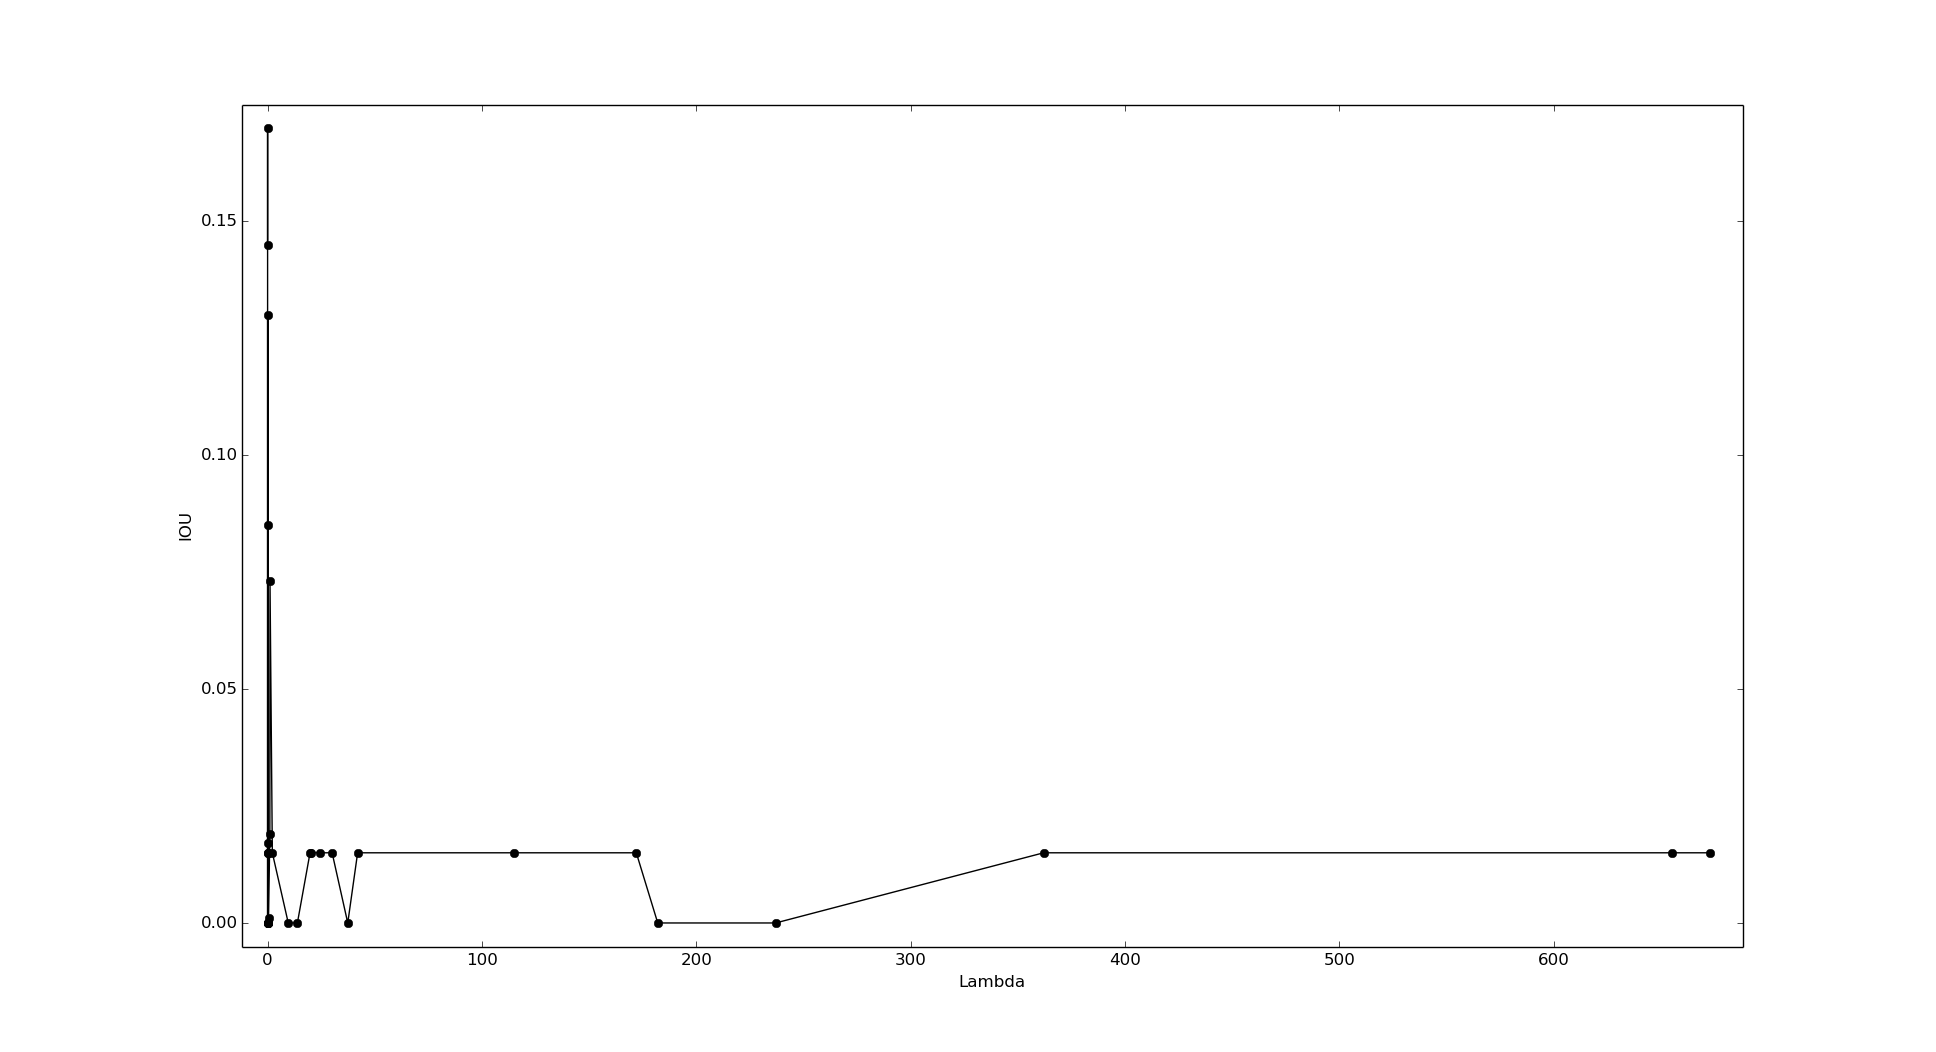
\includegraphics[width=\textwidth]{plots/hs1_lambda.png}
         \caption{IOU vs $\lambda$}
	\end{subfigure}
	\begin{subfigure}{0.32\textwidth}
		\centering
                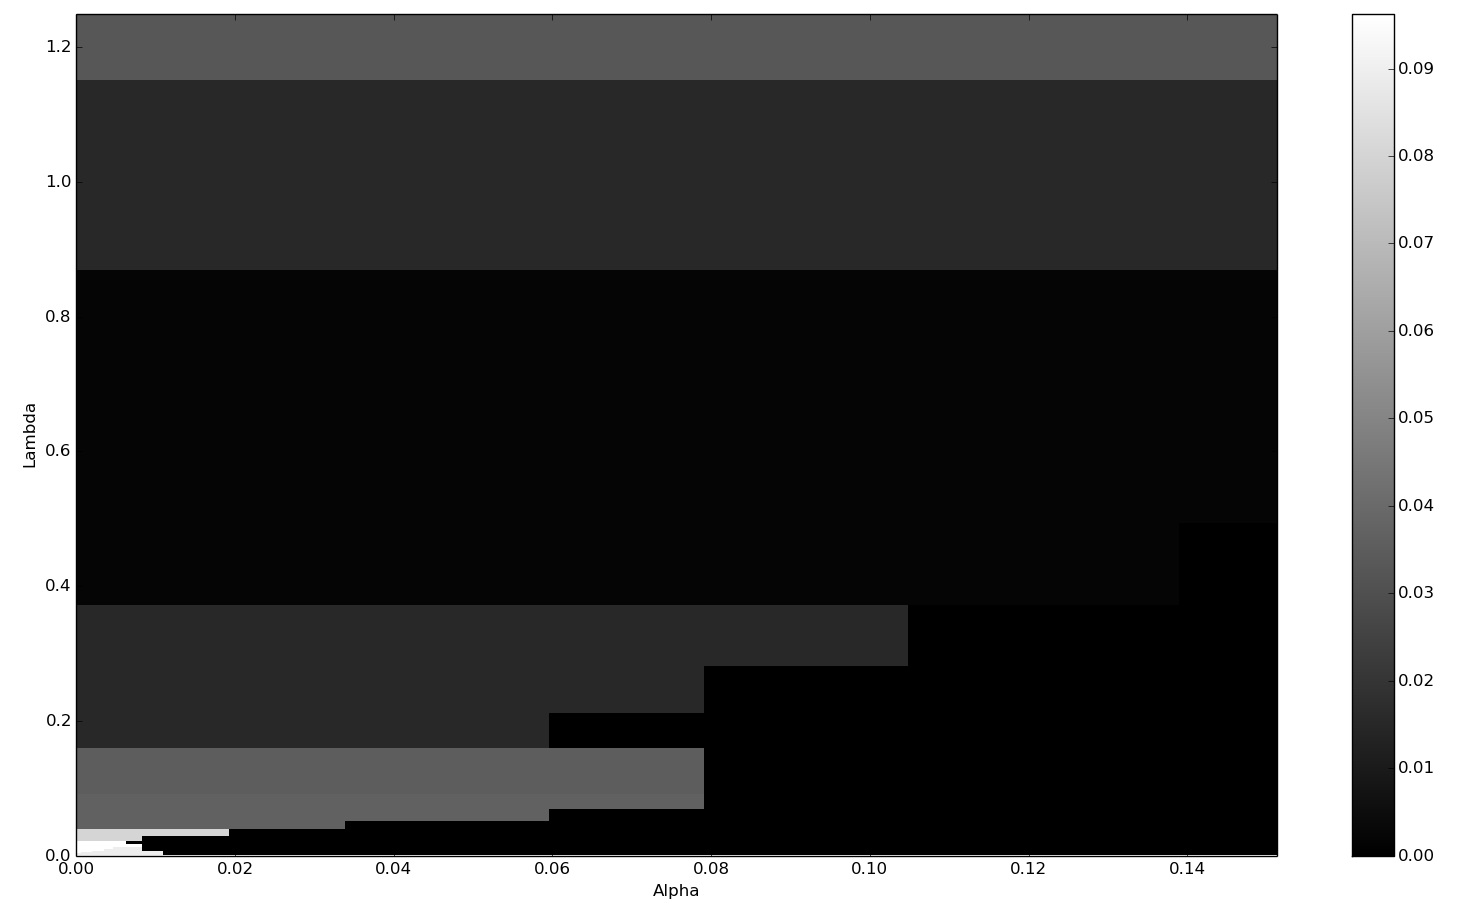
\includegraphics[width=\textwidth]{plots/hs1_pcolor.png}
         \caption{IOU (color) vs $\alpha$ (x) vs $\lambda$ (y)}
	\end{subfigure}
	\caption[First hyperparameter search for Experiment 1]{Results of the first search of hyperparameters. High IOU is better.}
	 \label{fig:Hs1}
\end{figure}

% Discussion: Divergenece and it can be also observed that lambda is not as important as alpha.
After refining the search range we had a better idea of which combinations produced the best results (Fig.~\ref{fig:Hs2}).
\begin{figure}[h]
	\centering
	\begin{subfigure}{0.32\textwidth}
		\centering
                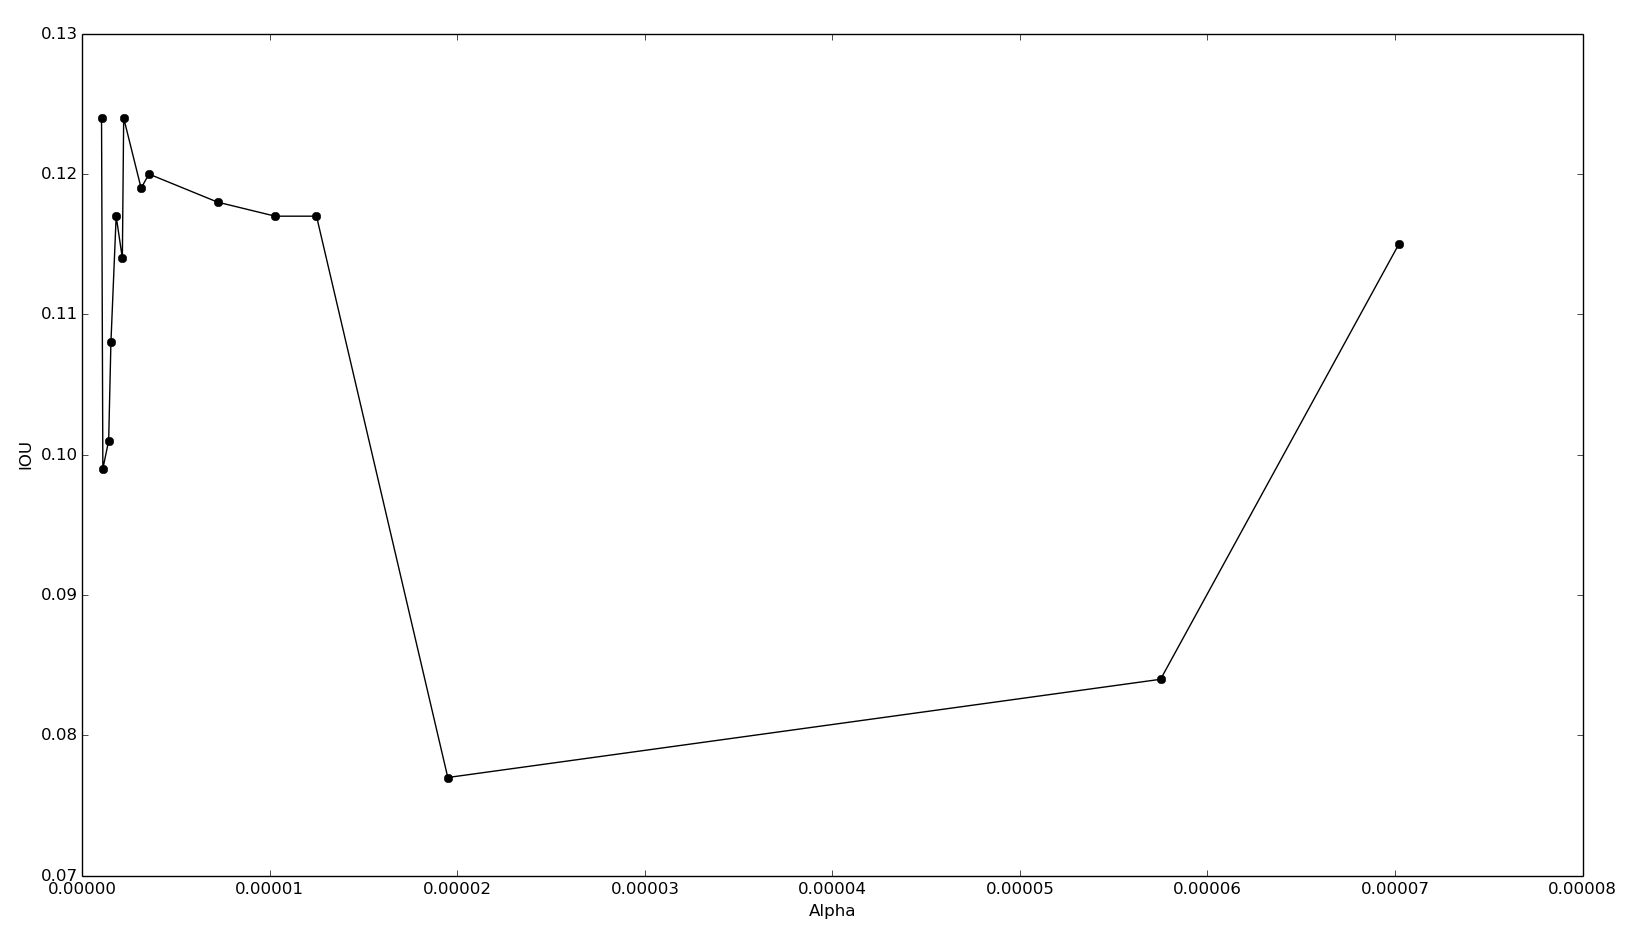
\includegraphics[width=\textwidth]{plots/hs2_alpha.png}
         \caption{IOU vs $\alpha$}
	\end{subfigure}
	\begin{subfigure}{0.32\textwidth}
		\centering
                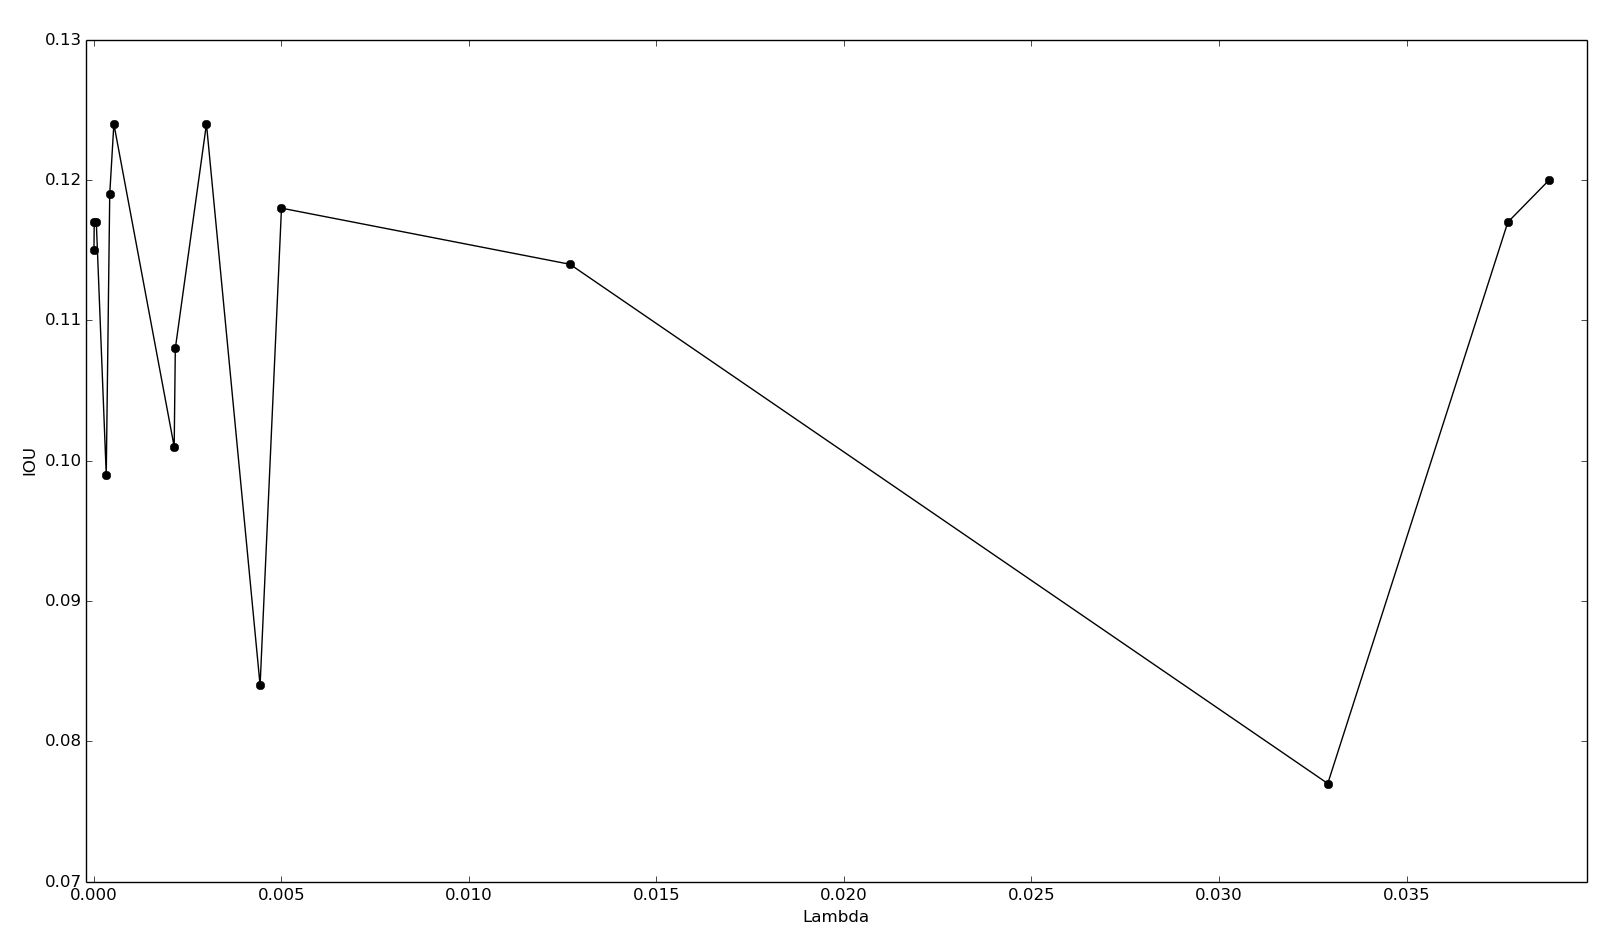
\includegraphics[width=\textwidth]{plots/hs2_lambda.png}
         \caption{IOU vs $\lambda$}
	\end{subfigure}
	\begin{subfigure}{0.32\textwidth}
		\centering
                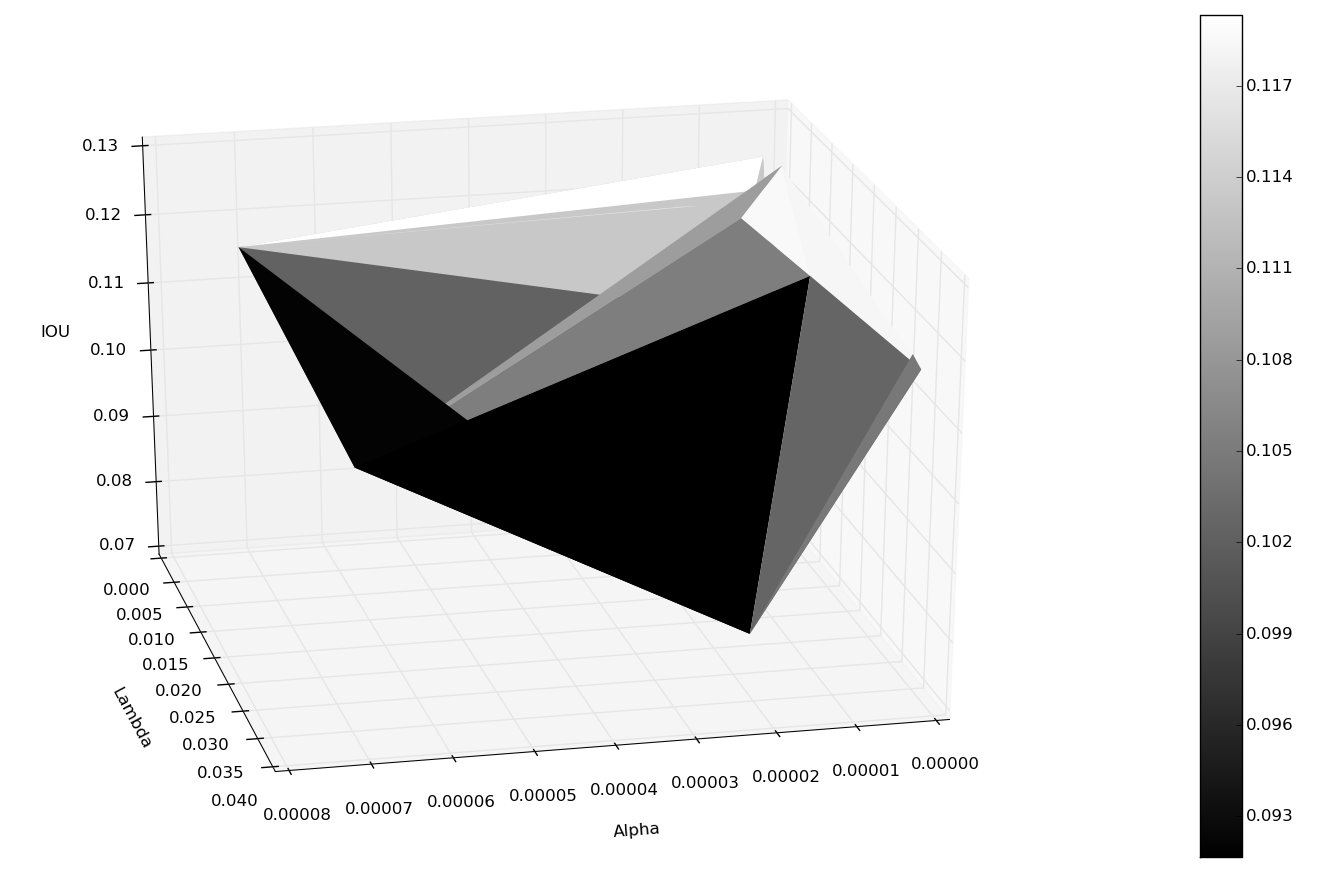
\includegraphics[width=\textwidth]{plots/hs2_trisurface.png}
         \caption{IOU (z) vs $\alpha$ (x) vs $\lambda$ (y)}
	\end{subfigure}
	\caption[Second hyperparameter search for Experiment 1]{Results of the second search of hyperparameters. High IOU is better.}
	 \label{fig:Hs2}
\end{figure}

With this results, we chose to train a network with $\alpha = 0.000004$ and $\lambda = 0.0008$.

\subsection{Evaluation}
After training the network, we used the validation set to select the best threshold: a 0.8 probability threshold (equivalent to 0.602 logit) produced the best IOU (0.133) in the validation set.

The test set results are summarized in Table~\ref{tab:Results1}
\begin{table}[h]
	\centering
	\begin{tabular}{cccccccc}
	\hline
	\textbf{IOU}	& \textbf{F1-score}	& \textbf{G-mean} &\textbf{Accuracy}	& \textbf{Sensitivity} & \textbf{Specificity} & \textbf{Precision} & \textbf{Recall}\\
	\hline
	0.022 & 0.031 & 0.038 & 0.975 & 0.028 & 0.982 & 0.040 & 0.028\\
	\hline
	\end{tabular}
	\caption[Results for Experiment 1]{Test results for the trained network (Sec~\ref{sec:Experiment1}).}
	\label{tab:Results1}
\end{table}

\subsection{Qualitative results}
We show the prediction and produced segmentation for some test examples.% in appendix A

%Images of original mammogram and label and predicitions (logits) and final segmentation

\section{Experiment 2}
\subsection{Hyperparameter search}
Similar to experiment 1, the best $\alpha$s and $\lambda$s were found in the bottom of the search range (Fig.~\ref{fig:Hs4}), however, performance is more robust to small changes. We show results only for the networks with the fifteen lowest $\alpha$s as bigger values caused training to diverge.
\begin{figure}[h]
	\centering
	\begin{subfigure}{0.32\textwidth}
		\centering
                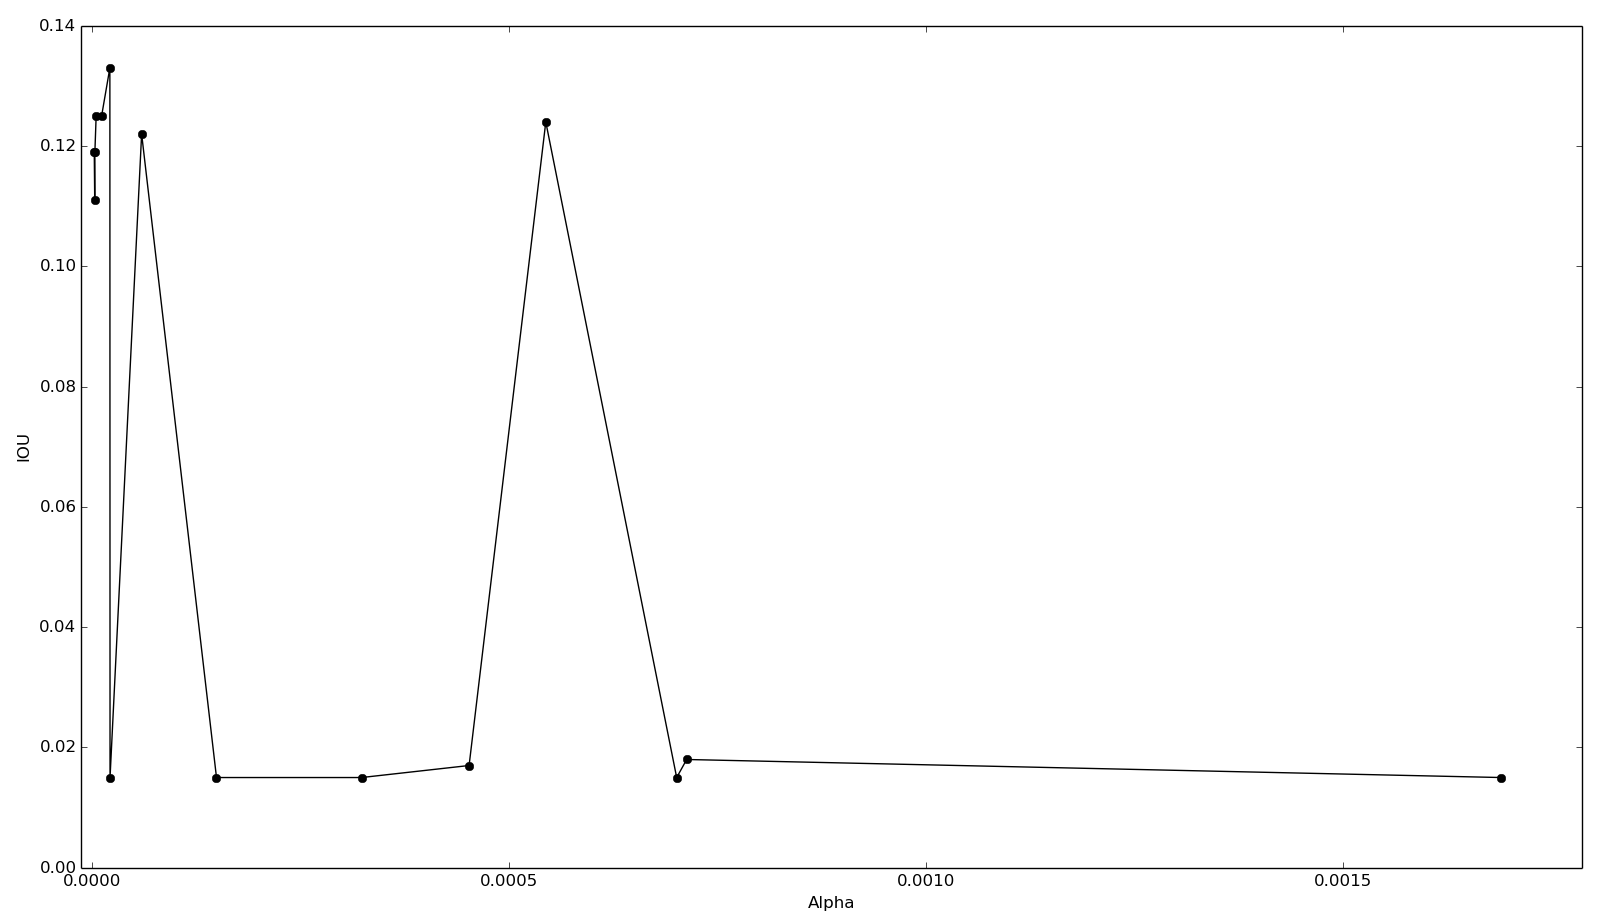
\includegraphics[width=\textwidth]{plots/hs4_alpha.png}
         \caption{IOU vs $\alpha$}
	\end{subfigure}
	\begin{subfigure}{0.32\textwidth}
		\centering
                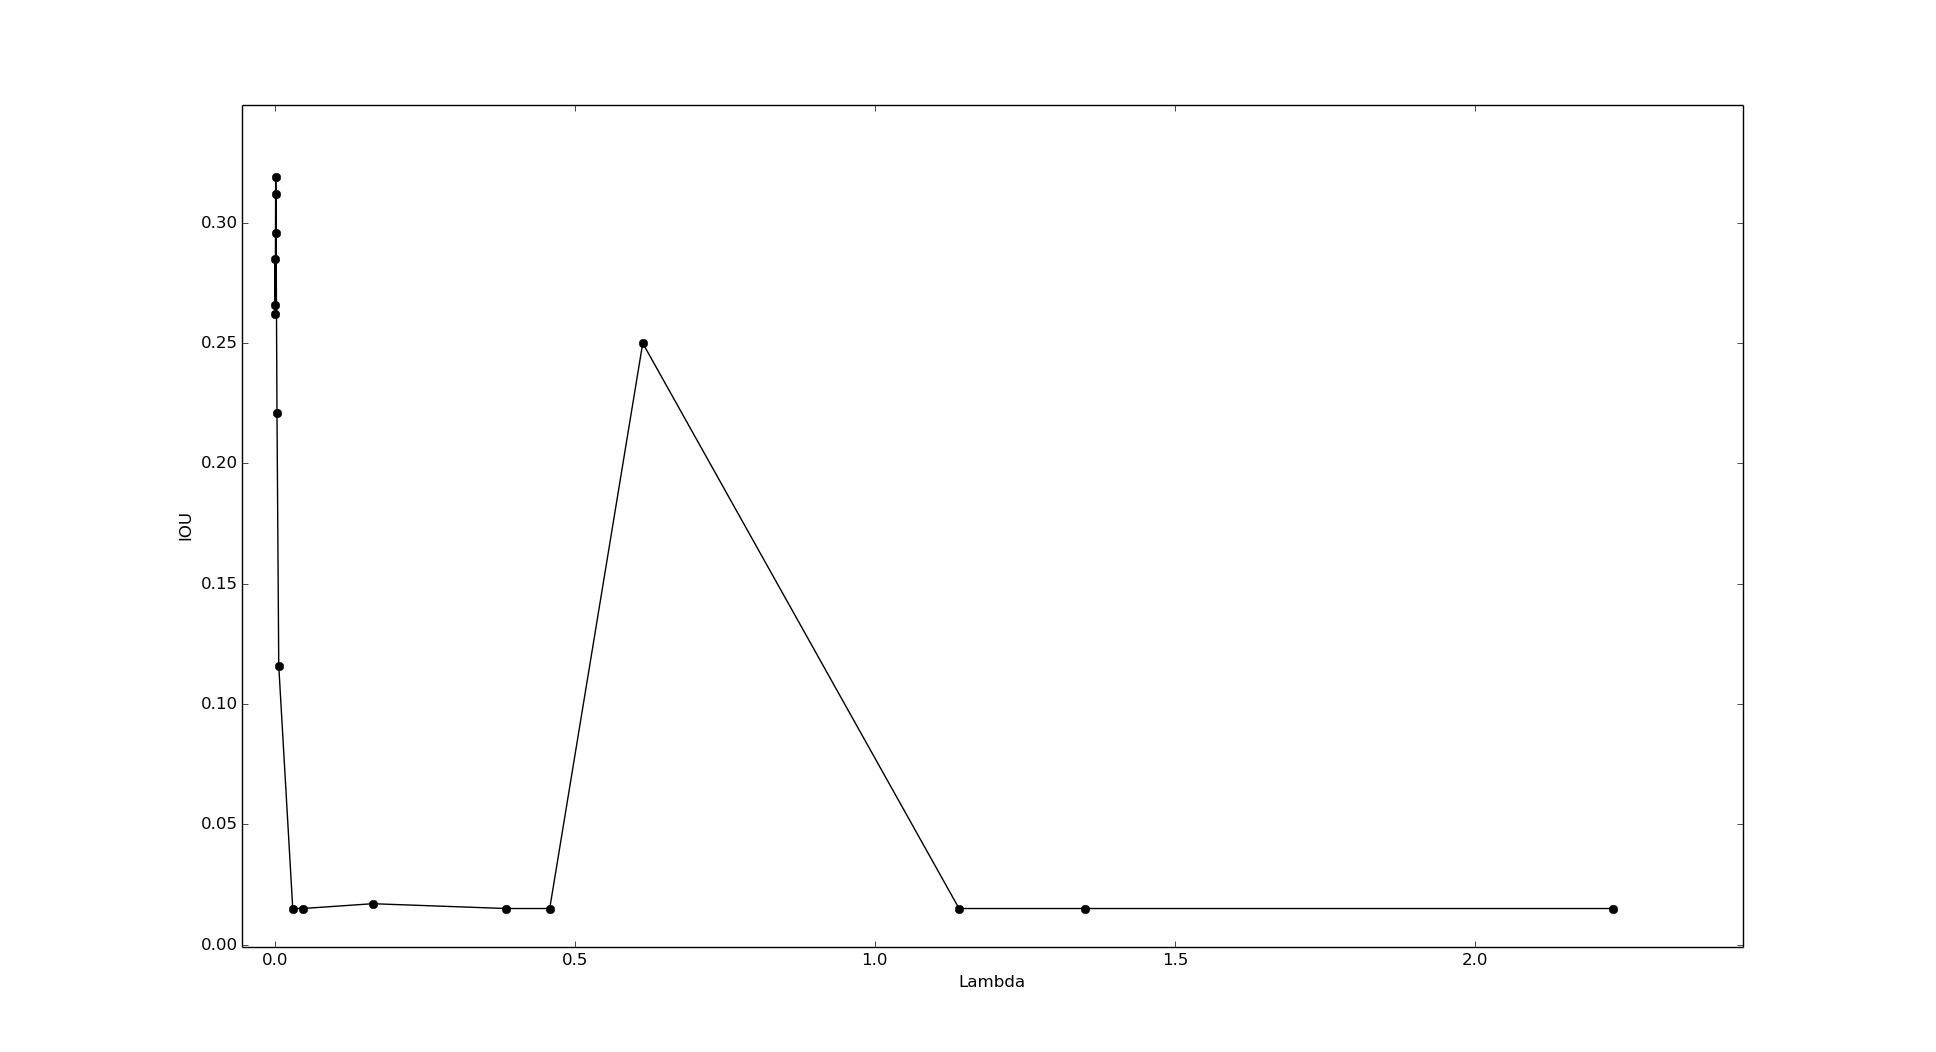
\includegraphics[width=\textwidth]{plots/hs4_lambda.png}
         \caption{IOU vs $\lambda$}
	\end{subfigure}
	\begin{subfigure}{0.32\textwidth}
		\centering
                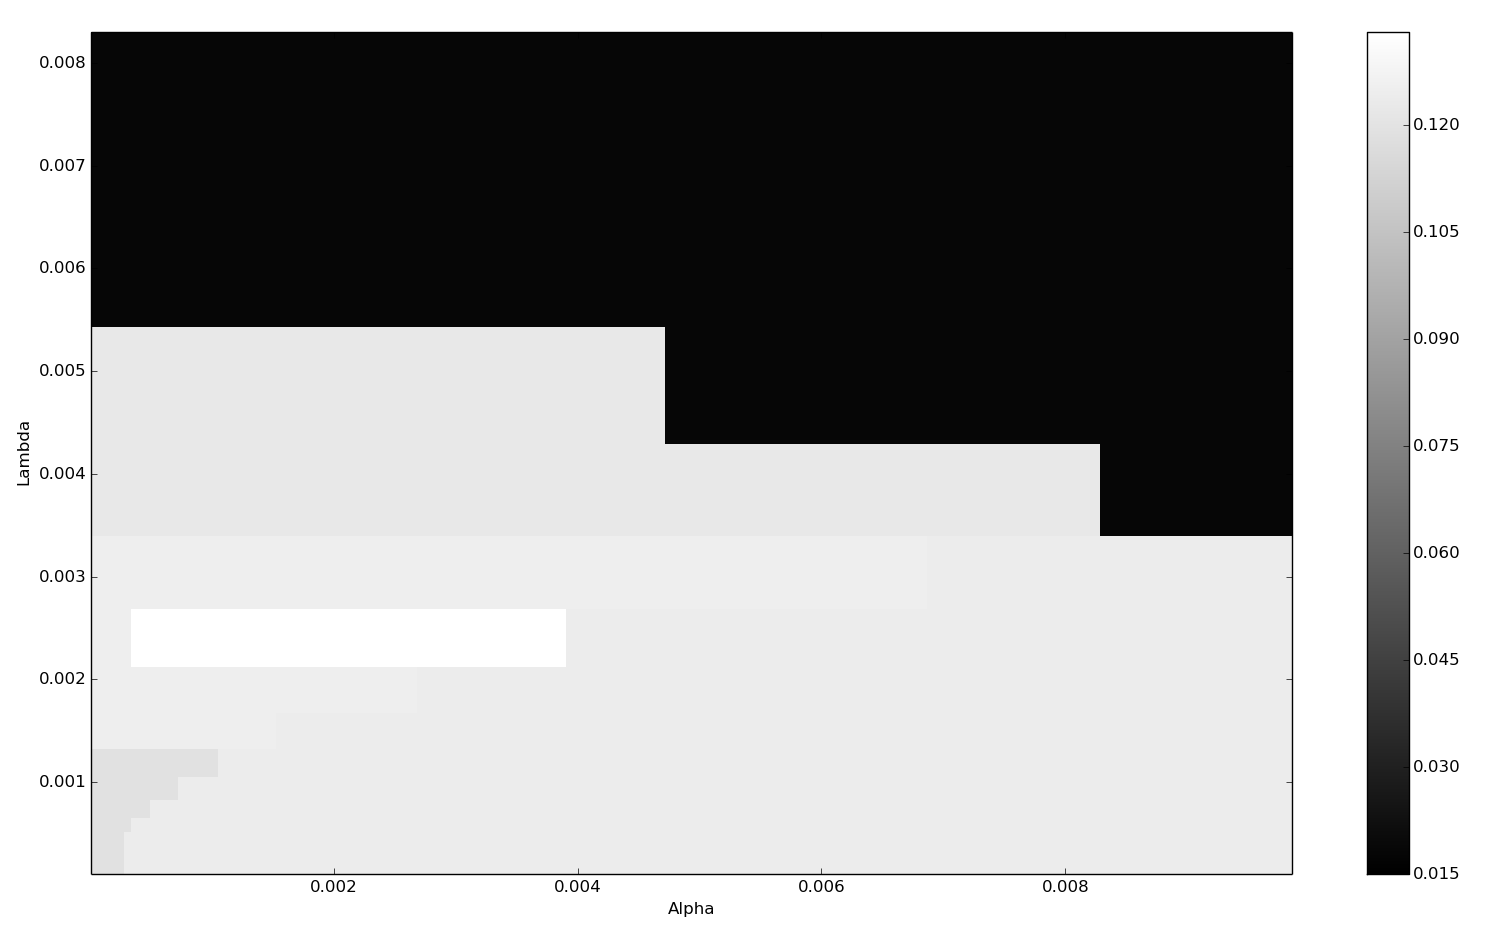
\includegraphics[width=\textwidth]{plots/hs4_pcolor.png}
         \caption{IOU (color) vs $\alpha$ (x) vs $\lambda$ (y)}
	\end{subfigure}
	\caption[Hyperparameter search for Experiment 2]{Results of the hyperparameter search. High IOU is better.}
	 \label{fig:Hs4}
\end{figure}

With this results we selected $\alpha = 0.00003$ and $\lambda = 0.002$ to train our network.

\subsection{Evaluation}

\subsection{Qualitative results}


\section{Discussion}
We found that....
